
% This LaTeX was auto-generated from MATLAB code.
% To make changes, update the MATLAB code and republish this document.

\documentclass{article}
\usepackage{graphicx}
\usepackage{color}

\sloppy
\definecolor{lightgray}{gray}{0.5}
\setlength{\parindent}{0pt}

\begin{document}

    
    
\section*{}


\subsection*{Contents}

\begin{itemize}
\setlength{\itemsep}{-1ex}
   \item a) Resolucion te�rica
   \item a) Grafico de comprobacion te�rico
   \item b)
   \item c) para encontrar el N
   \item c) para media y varianza
\end{itemize}


\subsection*{a) Resolucion te�rica}

\begin{verbatim}
p=0.01;
syms N
N=solve(0.5-(1-p)^N)
N=-log(2)/log(99/100)
\end{verbatim}

        \color{lightgray} \begin{verbatim} 
N =
 
-log(2)/log(99/100)
 

N =

   68.9676

\end{verbatim} \color{black}
    

\subsection*{a) Grafico de comprobacion te�rico}

\begin{verbatim}
clc, clear, close all
dir='G:\My Drive\AI\CURSO\prob_y_est_ia\examen\';
muestras=300;
X=1;
p=0.01;
% for X=1:10
for N=1:muestras
    a(N)=1-binocdf(0,N,p);
end
N=1:muestras;
plot(N,a)
xlabel('N');ylabel('1-binocdf(0,N,p)');
print('-depsc',[dir 'comprob_teo']);
hold on
grid on
% end
\end{verbatim}

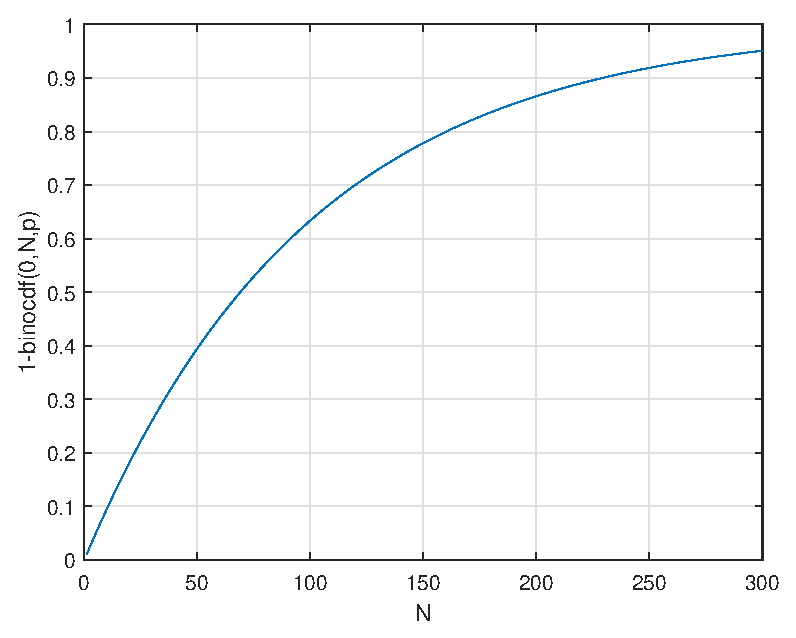
\includegraphics [width=4in]{ej_1_examen_01.eps}


\subsection*{b)}

\begin{verbatim}
N=68;
mu=N*p
sigma=sqrt(N*p*(1-p))
\end{verbatim}

        \color{lightgray} \begin{verbatim}
mu =

    0.6800


sigma =

    0.8205

\end{verbatim} \color{black}
    

\subsection*{c) para encontrar el N}



\subsection*{c) para media y varianza}

\begin{par}
proceso Bernoulli con v.a. uniforme
\end{par} \vspace{1em}
\begin{verbatim}
% configuro la semilla inicial del proceso aleatorio uniforme
rand ('seed', 123);

% probabilidad de fosforo defectuoso
p = 0.01;

% cantidad de fosforos por caja
n=68;

% numero de ensayos
N = 1e5;

% numero de cecas, vale 1 cuando es ceca
ndefectos_vector = zeros(N,1);

% se hacen N ensayos y en cada uno se guardan n fosforos en la caja, se
% buscan qu� cantidad de ellos son defectuosos con probabilidad p
for i = 1:N

  % n fosforos por ensayo
  for j = 1:n

    if(rand() < p)
      ndefectos_vector(i) = ndefectos_vector(i) + 1;
    end

  end

end

% calcular la media y varianza
media_muestral = sum(ndefectos_vector) / N

% varianza muestral
varianza_muestral = (1/(N-1)) * sum((ndefectos_vector - media_muestral * ones(N,1)).^2)

% media teorica
media_teorica = n*p

% varianza teorica
varianza_teorica = n * p * (1-p)
\end{verbatim}

        \color{lightgray} \begin{verbatim}
media_muestral =

    0.6760


varianza_muestral =

    0.6777


media_teorica =

    0.6800


varianza_teorica =

    0.6732

\end{verbatim} \color{black}
    


\end{document}
    
